\documentclass{article}

\usepackage{custom}
\usepackage{tikz}
\usetikzlibrary{positioning}
\usetikzlibrary{shapes,arrows}

\begin{document}

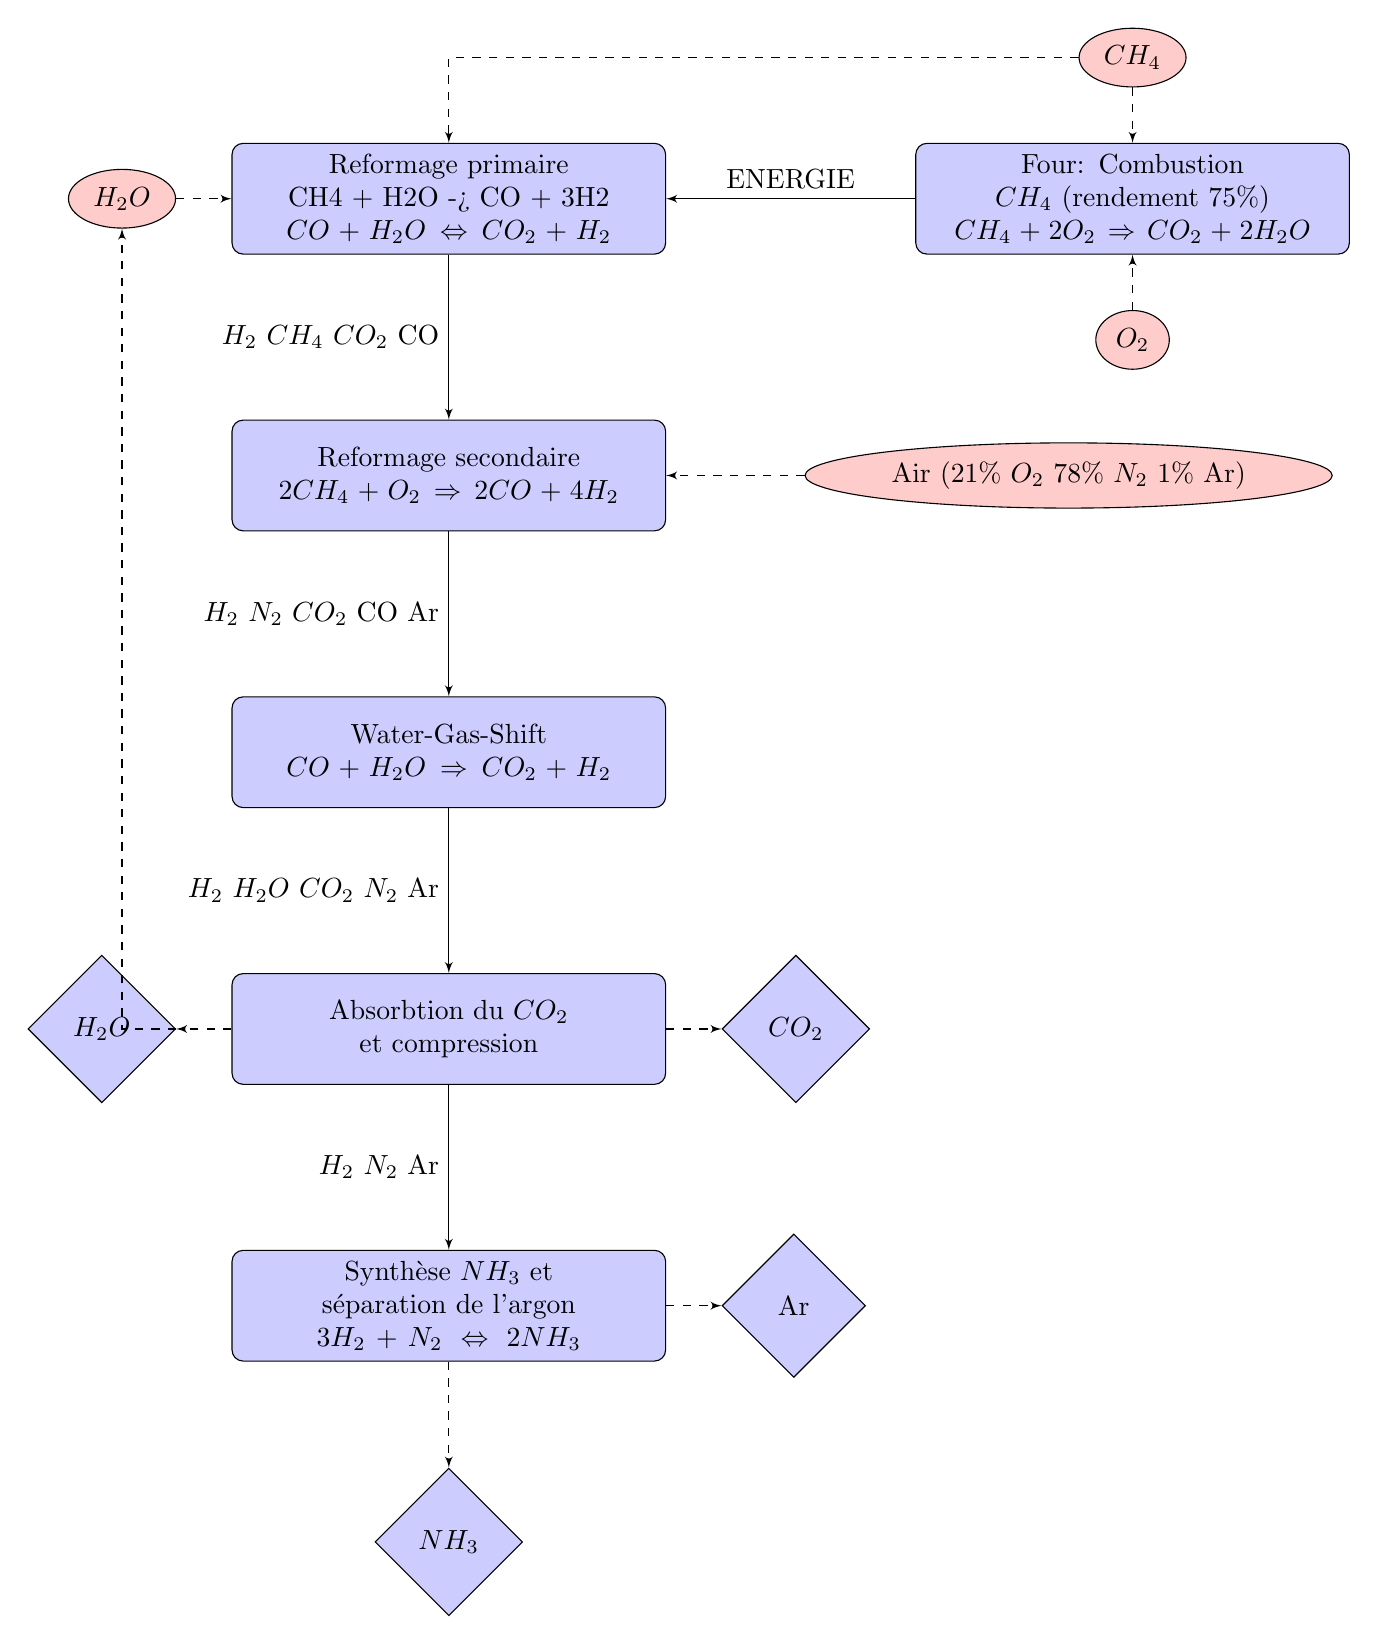
\begin{tikzpicture}
[node distance = 10em]

\tikzstyle{decision} = [diamond, draw, fill=blue!20, 
    text width=4.5em, text badly centered, node distance=3cm, inner sep=0pt]
\tikzstyle{block} = [rectangle, draw, fill=blue!20, 
    text width=15em, text centered, rounded corners, minimum height=4em]
\tikzstyle{line} = [draw, -latex']
\tikzstyle{cloud} = [draw, ellipse,fill=red!20, node distance=3cm,
    minimum height=2em]
    
\node [block] (primaire) {Reformage primaire \\
\ce{CH4 + H2O -> CO + 3H2} \\
$CO + H_2O \Leftrightarrow CO_2 + H_2$};
	\node [cloud, left = 2em of primaire] (H2O) {$H_2O$};
\node [block, right = 9em of primaire] (four) {Four: Combustion $CH_4$ (rendement 75\%) \\
$CH_4 + 2O_2 \Rightarrow CO_2 + 2H_2O$};
    \node [cloud, below = 2em of four] (O2) {$O_2$};
    \node [cloud, above = 2em of four] (CH4) {$CH_4$};
\node [block, below of=primaire] (secondaire) {Reformage secondaire \\
$2CH_4 + O_2 \Rightarrow 2CO + 4H_2$};
    \node [cloud, right = 5em of secondaire] (air) {Air (21\% $O_2$ 78\% $N_2$ 1\% Ar)};
\node [block, below of=secondaire] (wgs) {Water-Gas-Shift \\
$CO + H_2O \Rightarrow CO_2 + H_2$};
\node [block, below of=wgs] (abso) {Absorbtion du $CO_2$ et compression};
	\node [decision, right = 2em of abso] (CO22) {$CO_2$};
	\node [decision, left = 2em of abso] (H2O2) {$H_2O$};
\node [block, below of=abso] (synthese) {Synthèse $NH_3$ et séparation de l'argon \\
$3H_2 + N_2 \Leftrightarrow 2NH_3$};
	    \node [decision, below of=synthese] (NH3) {$NH_3$};
	    \node [decision, right = 2em of synthese] (argon) {Ar};


\path [line] (primaire) -- node[anchor = east] {$H_2$ $CH_4$ $CO_2$ CO}(secondaire);
\path [line] (four) -- node[anchor = south] {ENERGIE}(primaire);
    \path [line,dashed] (CH4) -- (four);
    \path [line,dashed] (CH4) -| (primaire);
    \path [line,dashed] (O2) -- (four);
\path [line] (secondaire) -- node[anchor = east] {$H_2$ $N_2$ $CO_2$ CO Ar}(wgs);
\path [line] (wgs) -- node[anchor = east] {$H_2$ $H_2O$ $CO_2$ $N_2$ Ar}(abso);
\path [line] (abso) -- node[anchor = east] {$H_2$ $N_2$ Ar}(synthese);
\path [line,dashed] (synthese) -- (NH3);
\path [line,dashed] (synthese) -- (argon);
\path [line,dashed] (air) -- (secondaire);
\path [line,dashed] (H2O) -- (primaire);
\path [line,dashed] (abso) -- (CO22);
\path [line,dashed] (abso) -- (H2O2);
\path [line,dashed] (H2O2) -| (H2O);

\end{tikzpicture}

\end{document}
